\documentclass{article}
\usepackage[final]{nips_2017}
\usepackage[utf8]{inputenc} % allow utf-8 input
\usepackage[T1]{fontenc}    % use 8-bit T1 fonts
\usepackage{hyperref}       % hyperlinks
\usepackage{url}            % simple URL typesetting
\usepackage{booktabs}       % professional-quality tables
\usepackage{amsfonts}       % blackboard math symbols
\usepackage{nicefrac}       % compact symbols for 1/2, etc.
\usepackage{microtype}      % microtypography
\usepackage{graphicx}
\title{Few-Shot Speaker Identification Using Masked Autoencoders and Meta-Learning}

\author{
  John Boccio \\
  Department of Electrical Engineering\\
  Stanford University\\
  \texttt{jboccio@stanford.edu} \\
  %% examples of more authors
  %% \And
  %% Coauthor \\
  %% Affiliation \\
  %% Address \\
  %% \texttt{email} \\
  %% \AND
  %% Coauthor \\
  %% Affiliation \\
  %% Address \\
  %% \texttt{email} \\
  %% \And
  %% Coauthor \\
  %% Affiliation \\
  %% Address \\
  %% \texttt{email} \\
  %% \And
  %% Coauthor \\
  %% Affiliation \\
  %% Address \\
  %% \texttt{email} \\
}

\begin{document}

\maketitle

\begin{abstract}
Speaker identification refers to the task of identifying which speaker is talking from a given set of 
speakers. With the rise of deep learning and data driven approaches to audio processing problems, new approaches can be
taken on this problem which traditionally was performed by trying to find separability between
speakers using hand-engineered feature extractors. The speaker identification problem is a very appropriate problem for meta-learning. 
Meta learning is a machine learning technique in which a model is trained to learn how to learn, allowing it to 
adapt to new tasks quickly using relatively little data. By applying meta-learning to the speaker identification problem, 
a model can be trained to learn how to recognize speakers from a small amount of audio samples from each of the speakers. 
This could be useful in scenarios where the set of possible speakers is not known in advance, or where the speakers may vary over time.
\\
\\
All of the data that was used for this paper comes from the VoxCeleb dataset \cite{DBLP:journals/corr/NagraniCZ17}. VoxCeleb
provides labeled audio data spoken from over 1,000 celebrities. These audio files are then cut into 3 second segments and 
converted into a spectrogram which will then be fed into a convolutional neural network. The final
result is a dataset with over 200,000 spectrograms, each labeled with an id that represents the celebrity that is talking.
\\
\\
The approach that this paper has taken towards applying meta-learning to the speaker identification problem is through the 
use of a prototypical network (protonet) \cite{DBLP:journals/corr/SnellSZ17}. The protonet generates an representation of a
spectrogram from one speaker which, ideally, is a far distance from the representation of a spectrogram from a different
speaker. These representations of each speaker are then used to perform classification. This paper also experiments with 
the affects of pretraining the network using a masked autoencoder \cite{DBLP:journals/corr/abs-2111-06377}. When applied to speaker identification, 
a masked auto encoder can be trained to extract characteristics of a speaker's voice from audio samples and use these 
characteristics to identify the speaker. Combining meta learning with masked auto encoders offers the potential to train 
a speaker identification model that can adapt to new speakers quickly and accurately using a small amount of training data. 
\\
\\
Given 5 examples of 5 different speakers, a model trained from scratch is able to identify who from these 5 speakers is
talking with 94\% accuracy. When the model is initialized with the weights learned from the masked autoencoder, the best
accuracy achieved decreased to 91\%.

\end{abstract}

\section{Introduction}
The problem that this paper is solving is the problem of speaker identification; given a set of speakers, create an
algorithm to identify which one of those speakers is speaking in an audio clip. This problem has a wide variety of 
applications ranging from security, automatic speech recognition, and forensic analysis. 

% Explain the problem and why it is important. Discuss your motivation for pursuing this
% problem. Give some background if necessary. Clearly state what the input and output
% is. Be very explicit: “The input to our algorithm is an {image, amplitude, patient age,
% rainfall measurements, grayscale video, etc.}. We then use a {SVM, neural network, linear
% regression, etc.} to output a predicted {age, stock price, cancer type, music genre, etc.}.”
% This is very important since different teams have different inputs/outputs spanning different
% application domains. Being explicit about this makes it easier for readers. If you are using
% your project for multiple classes, add a paragraph explaining which components of the
% project were used for each class.

\section{Related work}
There are multiple ways to tackle this problem and how you do so can depend on the data that you have available and 
the use case. If all of the speakers that need to be identified are known ahead of time and that set of speakers will 
not change, then a large network could be created to perform the classification. This approach is quite fragile as it 
depends on knowing all the potential speakers ahead of time, having plently of data for each, and restricts you to 
always classifying from your entire speaker set. Another approach is to form i-vectors \cite{ivectors}. An i-vector
is a representation of an utterance that is formed by utilizing a statisical model and speech-to-text. Characteristic 
information about a speaker's voice is contained within these i-vectors which can then be applied to the speaker 
identification task. This approach works well in some scenarios but still falls short as the i-vector may not be optimal
for finding separability between speakers even though it captures the characteristics of a speakers voice.

The shortcomings of classifying all speakers and using i-vectors can be resolved by using meta-learning. 

% You should find existing papers, group them into categories based on their approaches,
% and discuss their strengths and weaknesses, as well as how they are similar to and differ
% from your work. In your opinion, which approaches were clever/good? What is the stateof-the-art?
% Do most people perform the task by hand? You should aim to have at least
% 5 references in the related work. Include previous attempts by others at your problem,
% previous technical methods, or previous learning algorithms. Google Scholar is very useful
% for this: https://scholar.google.com/ (you can click “cite” and it generates MLA, APA,
% BibTeX, etc.)

\begin{figure}
  \centering
  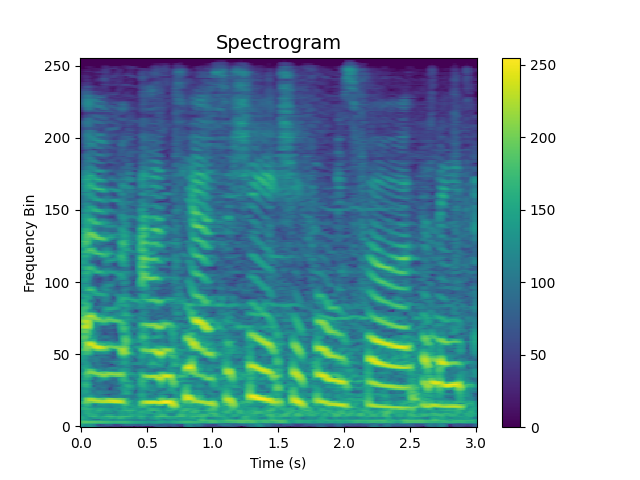
\includegraphics[width=0.6\textwidth]{Images/spectrogram_example.png}
  \caption[]{Spectrogram Captured from 3 Seconds of Speech}
  \label{fig:SpectrogramExample}
\end{figure}

\section{Dataset and Features}
The dataset used for this paper consists entirely of data from VoxCeleb \cite{DBLP:journals/corr/NagraniCZ17}. The 
VoxCeleb dataset is a collection of over 150,000 utterances from 1,251 celebrities. There is also the VoxCeleb2 \cite{Chung18b} 
dataset, which has even more celebrities and utterances, but VoxCeleb1 provided enough data for the purposes of this paper.
The owners and maintainers of VoxCeleb no longer host a download for all of the audio files of the utterances but the 
links to the youtube videos with labeled timestamps is available. A tool had to be created to scrape the data off of
youtube to reconstruct this dataset. The final result is a few thousand audio files, each of which have associated labeled
timestamps that specify which celebrity was speaking.

\subsection{Audio Preprocessing}
To preprocess the audio data from the VoxCeleb1 dataset, the raw audio data was converted into a melspectrogram. A 
spectrogram is a visual representation of the frequency content of a signal over time, and it can be useful for 
analyzing the characteristics of a speaker's voice. A melspectrogram, on the other hand, represents the audio data in 
terms of mel-frequency bins, which are a nonlinear scale of frequency that is closer to the way the human ear perceives 
sound. One advantage of using a melspectrogram instead of a regular spectrogram is that it can better capture the 
characteristics of the human voice, such as the pitch and timbre. This is because the mel-frequency scale is more closely 
aligned with the way the human ear processes sound, so a melspectrogram can better represent the spectral content of speech signals.

Since all of the utterances are of different lengths, a single length had to be decided on. In this paper, the 
length that was chosen was 3 seconds. If an utterance was greater than 3 seconds, then it was split into multiple 3 
second utterances. Any utterance that was less than 3 seconds was thrown out.

The Fast Fourier Transform (FFT) was used to convert the 3 seconds of audio data into the melspectrogram. The spectrogram
was created with 256 mels, 2048 point FFTs, a hanning windowing function, and a hop length equivalent to 10 milliseconds. 
All of the audio data was downloaded at a sample rate of 16 kHz, so a 10 millisecond hop length is equivalent to 160 
samples. The audio sampling rate being 16 kHz also implies that the maximum frequency of the spectrogram is 8 kHz which 
is enough to capture the large majority of speech sounds.

Once all the utterances are converted into melspectrograms, we arrive at a labeled dataset of over 250,000 images of 
size 256 by 301. This paper uses the same train and test split that is provided by VoxCeleb; 1,211 celebrities are in 
the training set and 40 celebrities are in the test set. The features in the melspectrograms provide the information
needed to create models that can perform speaker identification.

% Describe your dataset: how many training/validation/test examples do you have? Is there
% any preprocessing you did? What about normalization or data augmentation? What is the
% resolution of your images? How is your time-series data discretized? Include a citation on
% where you obtained your dataset from. Depending on available space, show some examples
% from your dataset. You should also talk about the features you used. If you extracted
% features using Fourier transforms, word2vec, PCA,
% ICA, etc. make sure to talk about it. Try to include examples of your data in the report
% (e.g. include an image, show a waveform, etc.).



\section{ Methods }
Describe your learning algorithms, proposed algorithm(s), or theoretical proof(s). Make
sure to include relevant mathematical notation. For example, you can include the loss function you are using. It is okay to use formulas from the lectures (online or in-class). For each algorithm, give a short description 
of how it works. Again, we are looking for your understanding of how these deep
learning algorithms work. Although the teaching staff probably know the algorithms, future
readers may not (reports will be posted on the class website). Additionally, if you are
using a niche or cutting-edge algorithm (anything else not covered in the class), you may want to explain your algorithm using 1/2
paragraphs. Note: Theory/algorithms projects may have an appendix showing extended
proofs (see Appendix section below).

\section{Experiments/Results/Discussion}
You should also give details about what (hyper)parameters you chose (e.g. why did you
use X learning rate for gradient descent, what was your mini-batch size and why) and how
you chose them. What your primary metrics are: accuracy, precision,
AUC, etc. Provide equations for the metrics if necessary. For results, you want to have a
mixture of tables and plots. If you are solving a classification problem, you should include a
confusion matrix or AUC/AUPRC curves. Include performance metrics such as precision,
recall, and accuracy. For regression problems, state the average error. You should have
both quantitative and qualitative results. To reiterate, you must have both quantitative
and qualitative results! If it applies: include visualizations of results, heatmaps,
examples of where your algorithm failed and a discussion of why certain algorithms failed
or succeeded. In addition, explain whether you think you have overfit to your training set
and what, if anything, you did to mitigate that. Make sure to discuss the figures/tables in
your main text throughout this section. Your plots should include legends, axis labels, and
have font sizes that are legible when printed.

\section{Conclusion and Future Work}
Summarize your report and reiterate key points. Which algorithms were the highestperforming?
Why do you think that some algorithms worked better than others? For
future work, if you had more time, more team members, or more computational resources,
what would you explore?

\section{Contributions}
John Boccio was the only member of the team and completed all of the work described in this report.

\bibliographystyle{plain}
\bibliography{refs}

\end{document}